\documentclass[11pt,a4paper]{article}
\usepackage[utf8]{inputenc}
\usepackage[margin=1in]{geometry}
\usepackage{graphicx}
\usepackage{hyperref}
\usepackage{xcolor}

\begin{document}
\noindent\textbf{\Large Tech Nation Visa - Exceptional Promise}\\
\noindent\textbf{Criteria:} Mandatory Criteria (Innovation) \& Optional Criteria 1/3 (Commercial Impact)\\
\noindent\textbf{Applicant:} Odeyemi Olusegun Israel\\
\rule{\textwidth}{0.4pt}

\vspace{0.5cm}
\begin{center}
    \textbf{\huge Evidence 3: UK Patent Application (IPO Filing)}
\end{center}
\vspace{0.5cm}

\section*{1. UK Intellectual Property Filing}
To protect the advanced machine learning architecture and cryptographic integration driving the AMTTP system, I filed a UK patent application via the Intellectual Property Office (IPO). This filing is evidence of commercial intent and of my effort to protect what I believe to be original technical work developed through the project.

\vspace{0.3cm}
\begin{center}
    \fbox{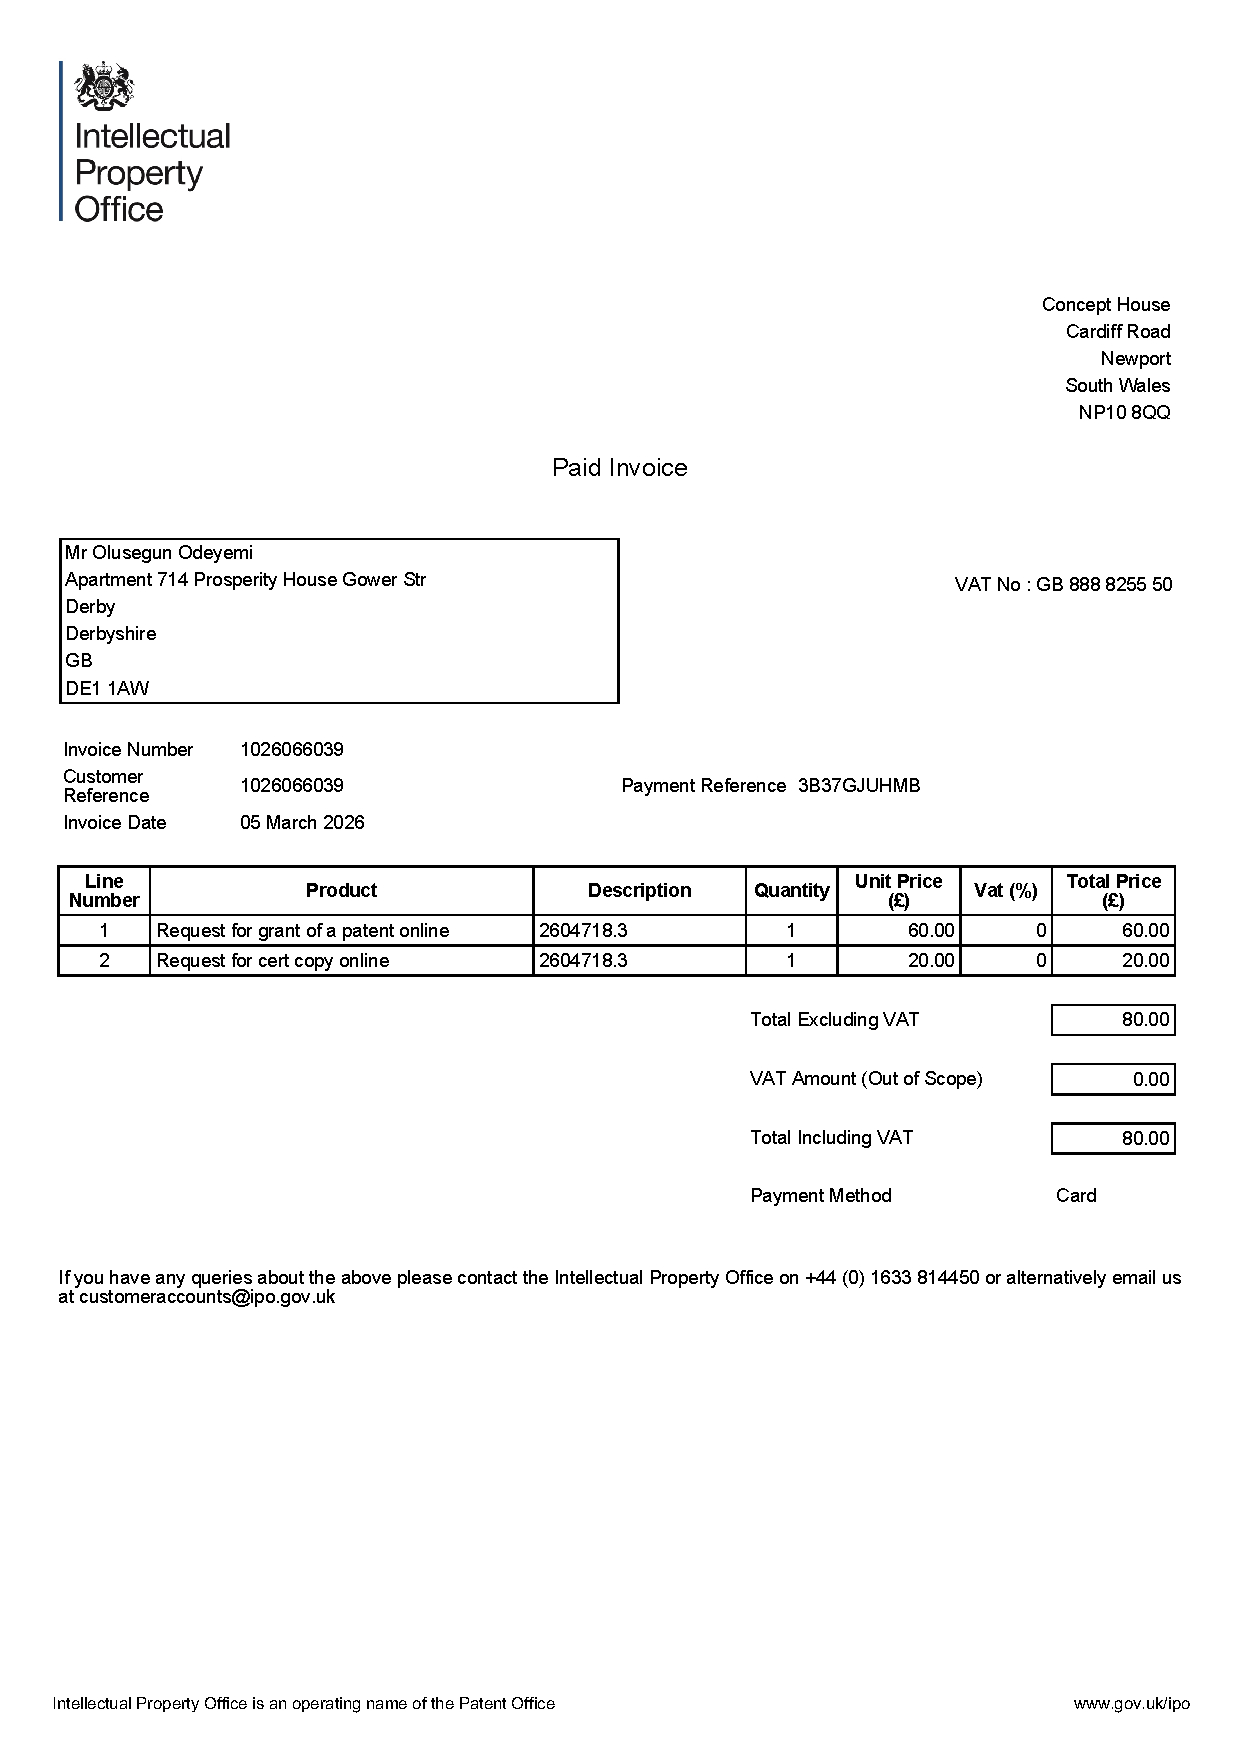
\includegraphics[width=0.88\textwidth, page=1]{images/ipo_receipt.pdf}}
\end{center}
\vspace{0.1cm}
\textit{Figure 1: Official UK IPO Patent Application Receipt (Application No. 1026066039) confirming intellectual property protection for the AMTTP compliance architecture.}

\section*{2. Summary of Technical Claims}
The patent explicitly covers the novel integration methodology where:
\begin{itemize}
    \item A distilled machine learning student model operates on an off-chain API Gateway to evaluate transaction risks in real-time.
    \item The off-chain risk score is securely bridged to EVM-compatible block-networks.
    \item Zero-Knowledge Proofs (ZK-SNARKs) interact with the Smart Contracts to finalize or revert transactions without leaking proprietary user PII on the public ledger.
\end{itemize}

\vspace{0.3cm}
\noindent\fbox{\begin{minipage}{0.95\textwidth}
\small
\textbf{Patent Abstract (Unified Application):} A unified system and method for detecting anomalies, scoring risk, enforcing compliance, and controlling stability across heterogeneous domains. The invention comprises eight subsystems:\\
\textbf{(1)} Blind-Spot Decomposition Theory --- four-channel diagnostic decomposition of classifier failures;\\
\textbf{(2)} Universal Deviation Principle --- multi-spectrum operator families with provable detection guarantees;\\
\textbf{(3)} GravityEngine --- N-body variational scoring with closed-form energy potentials;\\
\textbf{(4)} Dimension Magnifier --- boundary-centred nonlinear per-dimension transform;\\
\textbf{(5)} Risk-Aware Transaction Protocol (AMTTP) --- tiered escrow (Approve/Review/Escrow/Block), ML-oracle risk routing, zero-knowledge compliance verification, and cross-chain risk propagation;\\
\textbf{(6)} Adaptive Friction Framework --- Lyapunov-based adaptive friction for systemic risk detection;\\
\textbf{(7)} State-Dependent Viscosity --- transfers BSDT functional to computational fluid dynamics;\\
\textbf{(8)} UI Integrity Verification --- prevents interface manipulation attacks.
\end{minipage}}
\vspace{0.2cm}

\noindent\textit{Figure 2: Patent abstract detailing the eight core algorithmic subsystems protected under UK IPO Application No. 1026066039.}

\section*{3. Commercial Strategy}
This intellectual property filing supports my enterprise business strategy for AMTTP. It strengthens the platform's positioning as a scalable B2B infrastructure product that could be licensed to decentralised finance (DeFi) protocols and, in time, to regulated financial institutions seeking pre-settlement compliance tooling.

\end{document}